\section{时间反演对称}

分立的对称性除宇称(P,$x \to -x$)外,还有电荷共轭(C,$q \to -q$,即粒子$\to$反粒子),时间反演(T,$t \to -t$)。在弱相互作用中,单独的C对称,P对称,和联合的CP对称都不存在。必须加上T,联合的CPT对称存在。可以证明,点粒子必须满足联合的CPT对称和洛伦兹协变对称(CPT Theorem)。

本节将主要讨论时间反演对称。

\subsection{运动反演}

首先我们来做个“正名”的工作(所谓“名不正,则言不顺;言不顺,则事不成。”)。说“时间反演”\index{Time reversal:时间反演}(Time reversal)其实并不恰当,它会让人们误以为物理学家在讨论“回到过去”,“时空旅行”等,至少在这里我们所讨论的时间反演与这些是无关的。

就我们这里即将展开的讨论,更确切的名称应该是运动反演\index{reversal of motion:运动反演}(reversal of motion)。比如对经典力学,假设粒子在势场$V(x)$中运动,根据牛顿力学$F = m \ddot x = - \nabla V(x)$,我们求出粒子运动的轨迹$x(t)$。

所谓运动反演就是在某个特定的时刻,比如$t_0$,粒子的运动反向,$v \to - v$或$p \to -p$,我们发现$x(t)$仍然是$F = m \ddot x$的解,粒子运动的轨迹与运动反演前重合。我们称这种变换下的不变性称为运动反演对称,当然按物理学的常规术语,我们称其为时间反演对称。

%这里有一些标准的讨论,比如时间反演就相当于“倒着放”一段电影,在经典力学适用的场景下,只看影像运动,我们是无法断定影片是“正放”还是“倒放”的。这就是所谓时间反演对称。但对存在耗散(dissipation)的物理过程就不一样了,比如一个铅球落在一滩烂泥里,铅球的势能会转变为动能,动能最终会转变为热能,体现为烂泥和铅球温度的上升。对存在耗散的物理过程,熵是单边增大的($\Delta S \ge 0$)。据此我们很容易判别出哪段影片是“倒放”的(非物理的),而哪段影片是“正放”的(物理的)。

%比如我们可以设想一个人坐在玻璃房子里抽烟,最终烟尘将弥漫满整个房间,这是物理的。相反如果我们将此段影像“倒放”,我们将会看到充满整个房间的烟尘都逐渐聚集并“凝结”为一根香烟,这就是非物理的了。

%换句话说在以上过程中“正放”的影像对应一个物理法则(熵增),而“倒放”的影像对应一个非物理的法则(熵减)。

这里我们不讨论存在“耗散”\index{dissipation:耗散}(dissipation)的物理过程,仅指出两点:(1)“耗散”与一段时间有关,比如摩擦的发生总是要经历一段时间的,但时间反演则是发生在$t_0$瞬间的变换。(2)时间反演指的是在某特定时刻$t_0$,构成物理系统所有粒子的运动反演$v_i \to - v_i$或$p_i \to - p_i$(同时$x_i \to x_i$)。这暗示我们对系统信息的全盘和全部的掌握,但热力学的基本假设就是我们不可能具有此等对信息的全盘和全部掌握。由于适用条件的不同,我们不讨论如何把时间反演对称推广至包含耗散的物理过程。

这里我们提出两个任务:(1)如何把时间反演概念推广至电磁学;(2)如何把时间反演概念推广至量子力学。

电磁场的物理规律是麦克斯韦方程组\index{Maxwell equations:麦克斯韦方程组},

\begin{equation}
\nabla \cdot E = 4 \pi \rho, \nabla \times B - \frac{1}{c} \frac{\partial E}{\partial t} = \frac{4 \pi j}{c}, \nabla \times E = - \frac{1}{c} \frac{\partial B}{\partial t}
\end{equation}

带电粒子的运动方程由洛伦兹力\index{Lorentz Force:洛伦兹力}给定,

\begin{equation}
F = e \left( E + \frac{v \times B}{c}   \right)
\end{equation}

时间反演\index{Time reversal:时间反演}$t \to -t$,如果满足:

\begin{equation}
E \to E, B \to -B, \rho \to \rho, j \to -j, v \to -v
\end{equation}

可以验证此时麦克斯韦方程组和洛伦兹力的公式仍然成立。即我们有了某种变换下的不变性,这样我们就把时间反演概念推广到了电磁学的领域。(值得注意的是为了保证麦克斯韦方程组和洛伦兹力的公式不变,$t \to -t$变换的选择并不是唯一的,比如我们可以选择:$E \to -E$, $B \to B$, $\rho \to - \rho$, $j \to j$, $v \to -v$)

把时间反演概念推广到量子力学比较复杂,但有证据表明如果可以的话,时间反演和“取复共轭”这个操作有关。

考虑薛定谔方程(S.E.):

\begin{equation}
i \hbar \frac{\partial \psi}{\partial t} = \left( - \frac{\hbar^2}{2m}\nabla^2 + V \right) \psi
\end{equation}

假设$\psi(x,t) = u_n (x) e^{- i E_n t / \hbar}$是S.E.的解,那么$\psi(x, -t)$不是S.E.的解,但$\psi^* (x, -t)$就又是S.E.的解了。(这里我们假设对时间反演态,比如$\psi^* (x, -t)$,S.E.仍成立,就好像在经典力学中我们发现对$x(-t)$,牛顿方程仍成立。)

\subsection{反幺正算符}

以前我们讨论的种种对称变换都是幺正变换,这意味着当$\left| \alpha \right\rangle \to \left| \tilde{ \alpha }  \right\rangle$,$\left| \beta \right\rangle \to \left| \tilde{ \beta }  \right\rangle$,

\begin{equation}
\left\langle \beta | \alpha \right\rangle \to \left\langle \tilde{\beta} | \tilde{\alpha} \right\rangle = \left\langle \beta \right| U^\dagger U \left| \alpha \right\rangle = \left\langle \beta | \alpha \right\rangle 
\end{equation}

即态矢量的内积在幺正变换下是不变的。对量子力学而言,几率最终对应力学量的取值,几率对应内积的绝对值的平方。受此启发,我们试着把“态矢量的内积不变”这一要求稍稍放松。

\begin{equation}
\left|  \left\langle \tilde{\beta} | \tilde{\alpha} \right\rangle \right| = \left| \left\langle \beta | \alpha \right\rangle  \right|
\end{equation}

这意味着

\begin{equation}
\left\langle \tilde{\beta} | \tilde{\alpha} \right\rangle = \left\langle \beta | \alpha \right\rangle^* = \left\langle \alpha | \beta \right\rangle
\end{equation}

也是一种可能的选择。我们通过定义反幺正算符\index{Antiunitary operator:反幺正算符}$\theta$来兑现这种选择。

\begin{equation}
\left| \alpha \right\rangle \to \left| \tilde{\alpha} \right\rangle = \theta \left| \alpha \right\rangle, \left| \beta \right\rangle \to \left| \tilde{\beta } \right\rangle = \theta \left| \beta \right\rangle
\end{equation}

反幺正算符$\theta$可表示为幺正算符(U)作用于取复共轭算符(K)的形式:

\begin{equation}
\theta = UK
\end{equation}

反幺正算符满足如下性质:

\begin{eqnarray}
\left\langle \tilde{\beta} | \tilde{\alpha} \right\rangle  &  =  &  \left\langle \beta | \alpha \right\rangle^*  \\
\theta \left( c_1 \left| \alpha \right\rangle + c_2 \left| \beta \right\rangle \right) & = & c_1^* \theta \left| \alpha \right\rangle + c_2^* \theta \left| \beta \right\rangle 
\end{eqnarray}

这里需要注意,(2)对基矢$\left| a' \right\rangle$取复共轭仍然是$\left| a' \right\rangle$,

\begin{equation}
K \left| a' \right\rangle = \left| a' \right\rangle
\end{equation}

(2)另外对$\theta$而言,由于它是反幺正、反线性的,在算式中要把它看做是向右侧运算的。(Sakurai:it is always safer to work with the action of $\theta$on kets only. )我们也不试图去定义$\theta$的厄米共轭$\theta^\dagger$。

现在来证明对$\theta = UK$,$\left\langle \tilde{\beta} | \tilde{\alpha} \right\rangle  =  \left\langle \beta | \alpha \right\rangle^* $。

首先,

\begin{equation}
\left| \alpha \right\rangle = \sum\limits_{a'} \left| a' \right\rangle \left\langle a' | \alpha \right\rangle 
\end{equation}

对其施以反幺正变换,

\begin{equation}
\left| \tilde{\alpha} \right\rangle = UK \sum\limits_{a'} \left| a' \right\rangle \left\langle a' | \alpha \right\rangle = \sum\limits_{a'} U \left| a' \right\rangle \left\langle \alpha | a' \right\rangle
\end{equation}

类似地,对$\left| \tilde{\beta} \right\rangle$,

\begin{equation}
\left| \tilde{\beta} \right\rangle = UK \sum\limits_{a''} \left| a'' \right\rangle \left\langle a'' | \beta \right\rangle = \sum\limits_{a''} U \left| a'' \right\rangle \left\langle \beta | a'' \right\rangle
\end{equation}

因此:

\begin{eqnarray*}
\left\langle \tilde{\beta} | \tilde{\alpha} \right\rangle  & = & \sum\limits_{a' a''} \left\langle a'' | \beta \right\rangle \left\langle a'' \right| U^\dagger U \left| a' \right\rangle \left\langle \alpha | a' \right\rangle \\
{}  & = & \sum\limits_{a'} \left\langle \alpha | a' \right\rangle \left\langle a' | \beta \right\rangle = \left\langle \alpha | \beta \right\rangle
\end{eqnarray*}

\subsection{时间反演算符}

首先证明时间反演算符不可能是幺正算符,但可以是反幺正算符\index{Antiunitary operator:反幺正算符}。为了和一般的反幺正算符$\theta$区别开,我们把时间反演算符记为$\Theta$。

\begin{figure}[htbp]
\begin{center}
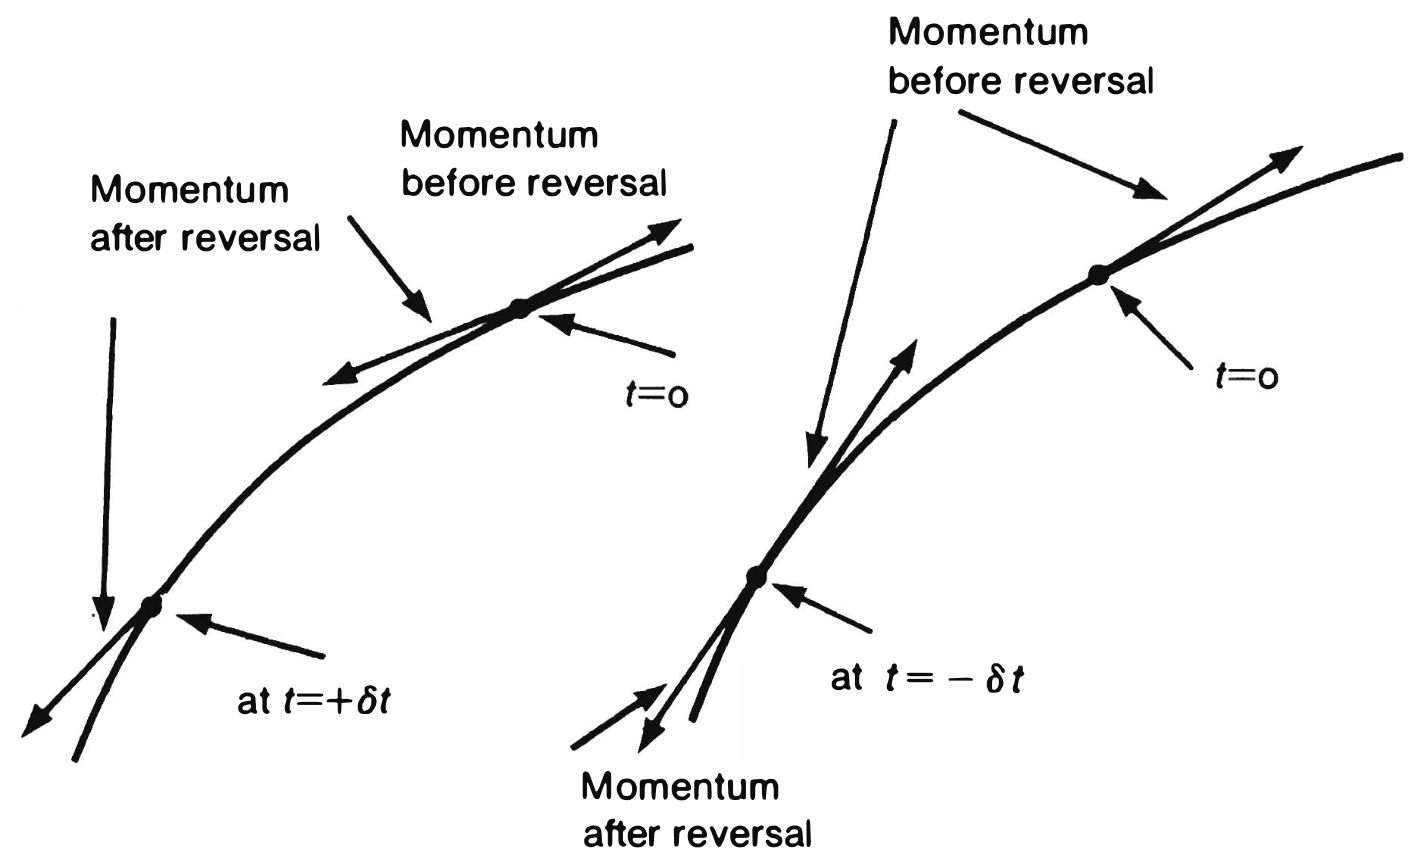
\includegraphics[width=10cm]{Symmetry/timereversal.png}
\caption{$ U(\delta t) \Theta \left| {} \right\rangle = \Theta  U(- \delta t) \left| {} \right\rangle $}
%\label{default}
\end{center}
\end{figure}

我们构造如图两个过程,这两个过程在效果上是相同的。左图对应的是先在$t=0$的时候时间反演\index{Time reversal:时间反演},时间反演后粒子的$p \to -p$,然后再演化$\delta t$,即粒子在$p$的延长线方向上运动$\delta t$时间,对应的量子态是:

\begin{equation}
U(\delta t) \Theta \left| {} \right\rangle
\end{equation}

右图对应的是先让粒子在动量$p$延长线的反方向上退行$\delta t$,然后再时间反演$\Theta$,对应的量子态是:

\begin{equation}
\Theta U(-\delta t) \left| {} \right\rangle  
\end{equation}

$\Theta \left| {} \right\rangle$是$\left| {} \right\rangle$的时间反演态。上述两个量子态相同,意味着:

\begin{equation}
U(\delta t) \Theta \left| {}  \right\rangle = \Theta U(-\delta t) \left| {} \right\rangle
\end{equation}

即:

\begin{equation}
\left( 1 -  \frac{i H \delta t}{\hbar}  \right) \Theta \left| {} \right\rangle = \Theta \left( 1 -  \frac{i H (- \delta t)}{\hbar}  \right) \left| {} \right\rangle
\end{equation}

这意味着:

\begin{equation}
- i H \Theta \left| {} \right\rangle  = \Theta i H \left| {} \right\rangle
\end{equation}

假设$\Theta$是幺正算符,我们可以把等式右侧的$i$直接提到$\Theta$前面去,于是得到:

\begin{equation}
- H \Theta = \Theta H
\end{equation}

但这会导致物理上无法接受的后果。

假设H的能量本征态$\left| n \right\rangle$($H \left| n \right\rangle = E_n \left| n \right\rangle$),

\begin{equation}
H \Theta \left| n \right\rangle = - \Theta H \left| n \right\rangle = - E_n \Theta \left| n \right\rangle
\end{equation}

这意味着$\Theta \left| n \right\rangle$也是H的本征态,且其能量本征值为$- E_n$。我们知道能量的取值是正定的($E \ge 0$),而$- E_n$意味着$E < 0$,这是物理上无法接受的结果。初等物理中喜欢说能量的取值依赖于能量零点的选择,但考虑到$E = m c^2$,能量就是质量,取负的能量意味着取负的质量,而负质量是非物理的,会导致很多奇怪的结果。总之在现有物理学框架内能量是不能小于0的。

假如$\Theta$是反幺正算符\index{Antiunitary operator:反幺正算符},$i$提出到最左边的时候就要加一个负号“-”,这意味着:

\begin{equation}
H \Theta = \Theta H
\end{equation}

对$\left| n \right\rangle$而言,

\begin{equation}
H \Theta \left| n \right\rangle = \Theta H \left| n \right\rangle = E_n \Theta \left| n \right\rangle
\end{equation}

即时间反演态$\Theta \left| n \right\rangle$对应的能量本征值仍是$E_n$,这样就不会导致任何不舒服了。

对宇称\index{Parity:宇称}$\pi$,我们说位置向量$x$在宇称下是奇的

\begin{equation}
\pi x \pi^\dagger = - x
\end{equation}

但这里我们无法定义$\Theta$的厄米共轭,我们使用$\Theta$的逆$\Theta^{-1}$,我们定义

\begin{equation}
\Theta A \Theta^{-1} = \pm A
\end{equation}

这里A是厄米算符,代表某力学量,我们称$\Theta A \Theta^{-1} = A$为时间反演变换下为偶的;而称$\Theta A \Theta^{-1} = - A$为时间反演变换下为奇的。

可以证明对时间反演态$\left| \tilde{\alpha}  \right\rangle$,

\begin{equation}
\left\langle \alpha \right| A \left| \alpha \right\rangle = \left\langle \tilde{\alpha} \right| \Theta A \Theta^{-1} \left| \tilde{\alpha} \right\rangle = \pm \left\langle \tilde{\alpha} \right| A \left| \tilde{\alpha} \right\rangle
\end{equation}

在时间反演下,我们期望动量$p$是奇的,位置$x$是偶的,即:

\begin{eqnarray}
\Theta p \Theta^{-1} & = & - p \\
\Theta x \Theta^{-1} & = & x
\end{eqnarray}

(1)假设$\left| p' \right\rangle$是动量$p$的本征态,那么$\left| p' \right\rangle$的时间反演态$\Theta \left| p' \right\rangle$对应的动量本征值是$- p'$。

动量$p$的本征值问题:

\begin{equation}
p \left| p' \right\rangle = p' \left| p' \right\rangle
\end{equation}

两侧都左乘$\Theta$

\begin{equation}
\Theta p \left| p' \right\rangle = \Theta p \Theta^{-1} \Theta \left| p' \right\rangle = - p \Theta \left| p' \right\rangle = p' \Theta \left| p' \right\rangle
\end{equation}

上式可改写为:

\begin{equation}
p \Theta \left| p' \right\rangle = - p' \Theta \left| p' \right\rangle
\end{equation}

即$\Theta \left| p' \right\rangle$对应的动量本征值为$-p'$。

(2)证明对一般的时间反演态$\Theta \left| {} \right\rangle$,基础对易式\index{fundamental commutation relation:基础对易式}$[x, p] = i \hbar$仍然成立。

首先把算符的等式写完整:

\begin{equation}
[x, p] \left| {} \right\rangle  = i \hbar \left| {} \right\rangle
\end{equation}

两侧都左乘$\Theta$

\begin{equation}
\Theta [x, p] \Theta^{-1} \Theta \left| {} \right\rangle = \Theta i \hbar \left| {} \right\rangle  
\end{equation}

上式可变化为

\begin{equation}
[x, -p] \Theta \left| {} \right\rangle = - i \hbar \Theta \left| {} \right\rangle
\end{equation}

即

\begin{equation}
[x, p] \Theta \left| {} \right\rangle = i \hbar \Theta \left| {} \right\rangle
\end{equation}

(3)假设$\Theta J \Theta^{-1} = -J$,我们可推出角动量的对易关系$[ J_x, J_y ] = i \hbar J_z $

首先:

\begin{equation}
[ J_x, J_y ] \left| {} \right\rangle = i \hbar J_z \left| {} \right\rangle
\end{equation}

两侧左乘$\Theta$

\begin{equation}
\Theta [ J_x, J_y ] \Theta^{-1} \Theta \left| {} \right\rangle = \Theta i \hbar J_z \left| {} \right\rangle
\end{equation}

上式可变化为

\begin{equation}
[ -J_x, -J_y  ] \Theta \left| {} \right\rangle = - i \hbar \Theta J_z \Theta^{-1} \Theta \left| {} \right\rangle
\end{equation}

化简后可得:

\begin{equation}
[J_x, J_y] \Theta \left| {} \right\rangle = i \hbar J_z \Theta \left| {} \right\rangle
\end{equation}

\subsection{自旋1/2的时间反演}

考察一个任意的自旋1/2的量子态——$\hat n$方向上取“+”的态——$\hat n$的取向用倾角$\beta$和方位角$\alpha$表示:

\begin{equation}
\left| n, + \right\rangle = e^{-i S_z \alpha / \hbar } e^{- i S_y \beta / \hbar} \left| + \right\rangle
\end{equation}

即通过对$\left| + \right\rangle$先围绕y轴转$\beta$再围绕z轴转$\alpha$来得到$\left| n, + \right\rangle$的量子态。

$\left| n, + \right\rangle$的时间反演态对应的是在$\hat n$方向上取“-”的量子态,考虑到相位的不确定,我们把它表示为:

\begin{equation}
\Theta \left| n, + \right\rangle = \eta  \left| n, - \right\rangle
\end{equation}

上式左侧可表示为:

\begin{eqnarray*}
\Theta \left| n, + \right\rangle  & = & \Theta e^{-i S_z \alpha / \hbar } e^{- i S_y \beta / \hbar} \left| + \right\rangle \\
{} & = & \Theta e^{-i S_z \alpha / \hbar } \Theta^{-1} \Theta e^{- i S_y \beta / \hbar} \Theta^{-1} \Theta \left| + \right\rangle \\
{} & = & e^{-i S_z \alpha / \hbar } e^{- i S_y \beta / \hbar}  \Theta \left| + \right\rangle
\end{eqnarray*}

因此:

\begin{equation}
e^{-i S_z \alpha / \hbar } e^{- i S_y \beta / \hbar}  \Theta \left| + \right\rangle = \eta e^{-i S_z \alpha / \hbar } e^{- i S_y (\beta + \pi) / \hbar} \left| + \right\rangle
\end{equation}

这意味着:

\begin{equation}
\Theta = \eta e^{- i S_y \pi / \hbar} K
\end{equation}

上式最后的K是必须放上去的,否则剩余部分就是个幺正算符了,这不符合时间反演算符是反幺正的这一性质。

利用:

\begin{equation}
e^{-i S_y \pi / \hbar } = - i \frac{2S_y}{\hbar}
\end{equation}

这样,我们求出对自旋1/2时间反演算符可表示为

\begin{equation}
\Theta = - i \eta \left( \frac{2 S_y}{ \hbar} \right) K = \eta K \left( \begin{array}{cc} 0 & -1  \\ 1 & 0 \end{array} \right) 
\end{equation}

下面,我们来证明对自旋1/2,有:$\Theta^2 = -1$。

考虑任意态矢量:

\begin{equation}
\chi = \left( \begin{array}{c} c_+  \\  c_- \end{array} \right)
\end{equation}

左乘$\Theta$

\begin{equation}
\Theta \chi = \eta K \left(  \begin{array}{c}  -c_-  \\ c_+  \end{array}  \right) =  \left(  \begin{array}{c}  - \eta c_-^*  \\  \eta c_+^*  \end{array}  \right)
\end{equation}

继续左乘$\Theta$

\begin{equation}
\Theta^2 \chi = \eta K \left(  \begin{array}{c} -\eta c_+^*  \\ - \eta c_-^* \end{array}  \right) = - \eta \eta^* \left( \begin{array}{c} c_+  \\  c_- \end{array} \right) = - \chi
\end{equation}

因此,

\begin{equation}
\Theta^2 = -1
\end{equation}

更一般地,我们能证明对角动量量子数j为半整数,$\Theta^2 = -1$,但对整数的j,$\Theta^2 = 1$(J. J. Sakurai, pp 278-279)。

\subsection{Kramers简并}

由$H \Theta = \Theta H$出发,由于$\Theta$是反幺正、反线性算符,所以我们无法从$H \Theta = \Theta H$得到一个守恒量。但由此式出发,我们可得到Kramers简并的概念。

假设$\left| n \right\rangle$是H的本征态,对应本征值是$E_n$,那么$\left| n \right\rangle$的时间反演态$\Theta \left| n \right\rangle$也是H的本征态,且对应本征值也是$E_n$。

假设对能级$E_n$不存在简并,即$\left| n \right\rangle$和$\Theta \left| n \right\rangle$本质上是一个量子态,二者间只差一个相位$\eta$,

\begin{equation}
\Theta \left| n \right\rangle = \eta \left| n \right\rangle
\end{equation}

这意味着:

\begin{equation}
\Theta^2 \left| n \right\rangle = \Theta \eta \left| n \right\rangle = \eta^* \eta \left| n \right\rangle = \left| n \right\rangle
\end{equation}

即$\Theta^2 =1 $,但我们知道对电子而言,自旋是1/2,这意味着$\Theta^2 $其实是$-1$。这说明时间反演态$\Theta \left| n \right\rangle $和$\left| n \right\rangle$是本质上不同的两个态,即$E_n$存在简并,我们称这种因时间反演不变导致的简并为Kramers简并\index{Kramers degeneracy:Kramers简并}。

容易证明对奇数个电子组成的系统存在Kramers简并,而对偶数个电子组成的系统不存在Kramers简并。外加磁场可将Kramers简并打开。

\subsection*{参考}

J. J. Sakurai, Modern Quantum Mechanics, \S 4.4